\chapter{Transformers in Computer Vision}

\noindent
No relevante.\\

\noindent
Las \tbf{redes recurrentes} (RNN) están diseñadas para procesar datos secuenciales (como texto o series temporales) donde el orden de los elementos importa. Formalmente se definen como 
\begin{itemize}
    \item \tbf{Generación de estados ocultos} ($h_t$): los modelos recurrentes generan de forma iterativa una secuencia de estados ocultos o vectores de memoria, representados como $h_t$
    \item \tbf{Función de transición}: cada estado oculto en el instante de tiempo actual $t$ se calcula como una función matemática dependiente de dos variables
    $$h_t = f(h_{t-1}, x_t)$$
    donde $h_{t-1}$ es el estado oculto del paso inmediatamente anterior (que idealmente condensa la información del pasado), y $x_t$ es el token o vector de entrada en la posición actual $t$ (por ejemplo, la palabra actual en una frase).
\end{itemize}

Los \underline{problemas} que tienen las RNN son:
\begin{itemize}
    \item \tbf{Pérdida de memoria a largo plazo}: a medida que la secuencia se hace más larga, las RNN tienen dificultades para mantener información relevante de los primeros elementos, lo que se conoce como el problema del \tbf{desvanecimiento del gradiente} (Vanishing Gradient). Esto significa que la influencia de los primeros tokens en la secuencia disminuye exponencialmente a medida que avanzamos en la secuencia, lo que dificulta el aprendizaje de dependencias a largo plazo.
    \item \tbf{Dificultad para paralelizar}: las RNN procesan los datos de forma secuencial, lo que significa que cada paso depende del resultado del paso anterior, es decir, el estado oculto $h_t$ depende de $h_{t-1}$.
\end{itemize}

\noindent
La solución a los problemas es añadir atención, de estas dos maneras
\begin{itemize}
    \item Reemplazar la recurrencia con \tbf{auto-atención} (self-attention), donde cada token puede atender a todos los demás tokens de la secuencia, lo que permite capturar dependencias a largo plazo sin importar la distancia entre los tokens.
    \item Eliminar las conexiones recurrentes, lo que permite un procesamiento completamente paralelo de la secuencia, mejorando significativamente la eficiencia computacional.
\end{itemize}
En esta sección nos basaremos en los \tbf{transformers}, que son un tipo de modelo de atención que ha revolucionado el campo del procesamiento del lenguaje natural (NLP) y se ha extendido a otras áreas como la visión por computadora. El transformer es una arquitectura de red sencilla basada en el mecanismo de atención que aumenta la velocidad con la que estos modelos pueden entrenar.

\section{Self Attention}
\noindent
El mecanismo de \tbf{self-attention} (auto-atención) es una técnica que permite a un modelo de aprendizaje automático asignar diferentes pesos a diferentes partes de la entrada al procesar una secuencia. En el contexto de los transformers, la auto-atención se utiliza para capturar las relaciones entre los tokens de una secuencia, independientemente de su posición relativa. Esto es especialmente útil para tareas como la traducción automática, el análisis de sentimientos y la generación de texto, donde la comprensión de las relaciones entre palabras es crucial. \\ \\

\noindent
Para entender la matemática, se utiliza la analogía de una búsqueda en una base de datos. Cada \underline{elemento} (token o patch de imagen) se proyecta dinámicamente en tres vectores distintos mediante matrices de pesos entrenables
\begin{itemize}
    \item \tbf{Query} ($Q$): representa lo que el elemento actual está ``buscando'' en los demás.
    \item \tbf{Key} ($K$): representa el ``índice'' o descripción de lo que ese elemento ofrece.
    \item \tbf{Value} ($V$): representa la información real que contiene el elemento y que se transmitirá si hay coincidencia.
\end{itemize}
estos vectores se calculan mediante multiplicaciones matriciales con matrices de pesos entrenables $W_Q$, $W_K$ y $W_V$ respectivamente. En la arquitectura del Transformer, antes de calcular la atención, la secuencia de entrada pasa por tres capas lineales independientes (capas de proyección o capas Dense/Linear sin función de activación). Cada una de estas tres capas lineales posee su propia matriz de pesos asociados. Esas tres matrices de pesos son, precisamente, $W_Q$, $W_K$ y $W_V$. \\

\noindent
Antes de que el modelo vea una sola imagen o palabra (al inicio del entrenamiento), las matrices no saben nada. Sus valores se generan mediante métodos de inicialización aleatoria (como la inicialización de Xavier/Glorot o He/Kaiming, que son estándares en Deep Learning para mantener la varianza de las activaciones controlada). \\ \\

\noindent
Veámos los pasos para calcular la atención
\begin{enumerate}
    \item Dado un token de entrada $x_i$, se proyecta a tres vectores: 
    $$q_i = W_Q x_i, \ k_i = W_K x_i \ \text{ y } \ v_i = W_V x_i$$
    \item Se calcula la puntuación de atención entre el token $i$ y cada token $j$ de la secuencia utilizando el producto escalar entre sus vectores de consulta ($q_i$) y clave ($k_j$): 
    $$s_{ij} = q_i^T k_j$$
    \item Escalar la puntuación de atención por $\sqrt{d_k}$ para estabilizar los gradientes durante el entrenamiento: 
    $$\hat{s}_{ij} = s_{ij} / \sqrt{d_k}$$
    donde $d_k$ es la dimensión de los vectores de clave.
    \item Aplicar la función softmax sobre las puntuaciones escaladas para obtener los pesos de atención: 
    $$a_{ij} = \text{softmax}_j(\hat{s}_{ij})$$ 
    lo que normaliza los pesos para que sumen 1.
    \item Agregar los valores ponderados para obtener el vector de contexto para el token $i$ 
    $$z_i = \sum_j a_{ij} v_j$$ 
    donde $z_i$ es el vector de contexto que representa la información relevante para el token $i$ basada en su atención a los demás tokens de la secuencia.
\end{enumerate}
Resumiendo los pasos anteriores, la fórmula de la atención se puede expresar de manera compacta en forma matricial como
\begin{equation*}
    \text{Attention}(Q, K, V) = \text{softmax}\left(\frac{QK^T}{\sqrt{d_k}}\right) V
\end{equation*} 
y se llama \tbf{Scaled Dot-Product Attention} (Atención por producto escalar escalado). En esta fórmula, $Q$, $K$ y $V$ son matrices que contienen los vectores de consulta, clave y valor para toda la secuencia, respectivamente. El producto $QK^T$ calcula las puntuaciones de atención para todos los pares de tokens, que luego se escalan y se normalizan con softmax antes de multiplicar por $V$ para obtener los vectores de contexto finales.

\begin{observacion}
    En cuanto a la \tbf{complejidad}, el cálculo de la atención tiene una complejidad de $O(n^2 d)$ en tiempo y $O(n^2)$ en memoria, donde $n$ es la longitud de la secuencia (número de tokens o parches) y $d$ es la dimensión de los vectores de consulta, clave y valor. Esto se debe a que se necesita calcular las puntuaciones de atención para cada par de tokens, lo que resulta en una matriz de atención de tamaño $n \times n$. Esta complejidad cuadrática es el principal cuello de botella para secuencias largas, como imágenes de alta resolución, donde el número de tokens puede ser muy grande.
\end{observacion}

\subsection{Multi-Head Attention}
\noindent
La intuición de este modelo es resolver una limitación crítica del bloque de autoatención simple (\tbf{Single-Head Attention}). En un mecanismo de atención único, el cálculo suele verse dominado por el propio token (es decir, una palabra o un píxel tiende a prestarse la mayor cantidad de atención a sí mismo) o se ve obligado a enfocarse en un único tipo de relación geométrica o semántica, ignorando otras que ocurren en paralelo. \\ \\

\noindent
En lugar de realizar una sola operación de atención gigante, el modelo divide el espacio y ejecuta $h$ cabezas de atención en paralelo. Cada cabeza ($i$) opera en su propio subespacio de representación porque posee su propio conjunto exclusivo de matrices de pesos entrenables: 
$$W_Q^{(i)}, \ W_K^{(i)} \ \text{  y } \ W_V^{(i)}$$
El proceso técnico consta de 3 pasos:
\begin{enumerate}
    \item \tbf{Computación en paralelo}: cada una de las $h$ cabezas calcula su propia matriz de atención utilizando la fórmula estándar de Scaled Dot-Product Attention que ya conocemos, generando un output independiente denominado $Z^{(i)}$
    $$Z^{(i)} = \text{Attention}(QW_Q^{(i)}, KW_K^{(i)}, VW_V^{(i)})$$
    Al final de este paso, tenemos $h$ vectores de salida diferentes ($Z^{(1)}, Z^{(2)}, \dots, Z^{(h)}$) para el mismo token.
    \item \tbf{Concatenación}: para poder continuar con el flujo de la red, no podemos tener los resultados fragmentados. El modelo une (concatena) espacialmente todos los vectores resultantes uno al lado del otro en una única matriz
    $$\text{Output Concatenado} = [Z^{(1)}, Z^{(2)}, \dots, Z^{(h)}]$$
    \item \tbf{Proyección Lineal Final}: la matriz concatenada es muy ``ancha'' computacionalmente. Para devolver el vector a su dimensión original de diseño ($d_{model}$) y permitir que la información de todas las cabezas se mezcle e interactúe de forma efectiva, se multiplica por una nueva matriz de proyección final entrenable, llamada $W^O$
    $$\text{MHA} = [Z^{(1)}, Z^{(2)}, \dots, Z^{(h)}]W^O$$
\end{enumerate}
Los \underline{beneficios} de la atención multi-cabeza son que cada cabeza puede enfocarse en diferentes tipos de relaciones (sintácticas, de coreferencia, de co-ocurrencia); efectivamente creando múltiples ``subespacios de representación''. Esto permite al modelo capturar una variedad más rica de patrones y relaciones en los datos. \\ \\

\noindent
Una cosa que no hemos tenido en cuenta en el modelo descrito hasta ahora es una forma de tener en cuenta el orden de las palabras en la secuencia de entrada. Para abordar esto, el transformer añade un vector a cada embedding de entrada que le ayuda a determinar la posición de cada palabra. Este vector se llama \tbf{positional coding} y se suma al embedding de cada token antes de ser procesado por las capas de atención, lo podemos ver en la Figura \ref{fig:positional_coding}. 

\begin{figure}[h]
    \centering
    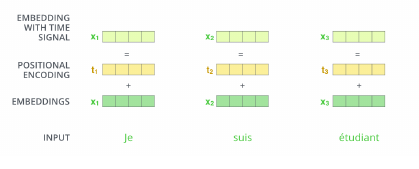
\includegraphics[width=0.8\textwidth]{img/positional_coding.png}
    \caption{Vector de control del orden de cada palabra.}
    \label{fig:positional_coding}
\end{figure}
Cada sub-layer (self-attention, feed forward neural net) en cada encoder tiene una \tbf{conexión residual} alrededor de él, y es seguido por un paso de normalización de capa (layer-normalization). Esto ayuda a estabilizar el entrenamiento y permite que la información fluya más fácilmente a través de las capas del modelo, mitigando problemas como el desvanecimiento del gradiente. \\

\noindent
En lugar de que una capa intente aprender directamente la representación ideal (llamémosla $H(x)$), la conexión residual obliga a la capa a aprender únicamente una función de residuo o modificación: $F(x) = H(x) - x$. Por lo tanto, la operación matemática exacta que ocurre en cada subcapa del bloque se define así:
$$\text{Salida} = x + F(x)$$
donde:$x$ es la identidad o información original que entra a la subcapa (viaja a través de la flecha que ``salta'' la capa por el lateral), y $F(x)$ es la transformación compleja computada por la subcapa (ya sea la atención o el MLP). \\

\begin{observacion}
    Una de las claves de usar los residuales es evitar el \tbf{desvanecimiento del gradiente}, que se basa en que si los valores de los pesos de las capas son menores que 1, al multiplicarlos tantas veces el gradiente se reduce exponencialmente hasta hacerse cero ($0$). Al llegar a las primeras capas del modelo, el gradiente ha desaparecido y la red deja de aprender. La solución matemática, viene al aplicar la derivada sobre la suma residual $\frac{\partial}{\partial x}(x + F(x))$, donde obtenemos
    $$\frac{\partial \text{Salida}}{\partial x} = 1 + \frac{\partial F(x)}{\partial x}$$
    ese número $1$ es mágico, pues garantiza que, incluso si la derivada de la capa compleja $\frac{\partial F(x)}{\partial x}$ se desvanece y se vuelve cero, el gradiente total siempre tendrá al menos un valor de $1$. El gradiente puede fluir directamente hacia atrás a través del ``atajo'' sin alterarse, permitiendo que todas las capas del modelo se entrenen correctamente.
\end{observacion}

\section{Tranformer Encoder}
\noindent
El bloque de encoder del transformer es fundamental porque representa la ``caja negra'' que recibe una secuencia de datos y la transforma en una representación matemática profundamente contextualizada. Vamos a explicar su arquitectura y funcionamiento. \\

\noindent
Cada transformer encoder, tiene varios bloques, que se ejecutan varias veces, pero todos tienen la misma estructura que viene dada en la Figura \ref{fig:transformer-encoder} y explicaremos a continuación
\begin{enumerate}
    \item \tbf{Multi-Head Attention (MHA)}: es el motor que ya estudiamos. Toma la secuencia y calcula las relaciones globales y simultáneas entre todos los tokens utilizando múltiples cabezas en paralelo.
    \item \tbf{Add \& Norm}: en esta capa se aplica normalización a la salida anterior y su suma con los residuales, lo que queda como
    \begin{equation*}
        x'=\text{LayerNorm}(x+MHA(x))
    \end{equation*}
    \item \tbf{Feed Forward Network} (FFN): una vez que la atención ha permitido que los tokens ``hablen entre sí'' e intercambien información, cada token pasa de forma independiente por una red neuronal densa. Dicha red neuronal suele ser dos capas con ReLu como función de activación, aplicada de forma posicional (es decir, cada token se procesa de forma independiente sin compartir información entre ellos en esta etapa).
\end{enumerate}

\begin{figure}
    \centering
    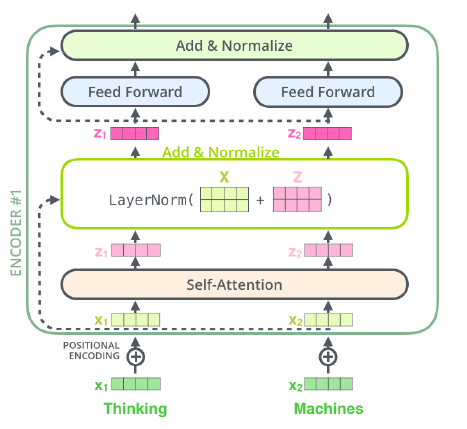
\includegraphics[width=0.8\textwidth]{img/transformer_encoder.png}
    \caption{Arquitectura de un bloque de encoder del transformer.}
    \label{fig:transformer_encoder}
\end{figure}

\section{Vision Transformer (ViT)}
\noindent
Si aqui intentasemos aplicar el transforemer de forma nativa a una imagen tratando cada píxel como si fuera una palabra (un token), la complejidad computacional colapsaría el hardware. Para una imagen estándar y pequeña de $256 \times 256$ píxeles, tenemos un total de $65.536$ píxeles, lo que resulta inviable. \\ \\
\noindent
La solución a este problema es dividir la imagen en parches (patches) de tamaño fijo, por ejemplo, $16 \times 16$ píxeles. Cada parche se trata como un token individual, lo que reduce drásticamente el número de tokens a procesar. 

\begin{observacion}
    Un \tbf{pipeline} (que se puede traducir como tubería o canalización de datos) se refiere a una secuencia ordenada y encadenada de pasos o bloques operativos donde la salida (output) de un componente se convierte directamente en la entrada (input) del siguiente. \\
\end{observacion}

\noindent
Veremos a continuación el pipeline completo de un Vision Transformer (ViT):
\begin{enumerate}
    \item \tbf{Patch extraction}: la imagen se divide en $N$ parches. El número total de parches se calcula con la fórmula
    $$N = \frac{H \times W}{P^2}$$
    el predeterminado es $P=16$.
    \item \tbf{Linear Projection}: cada parche bidimensional tiene un tamaño de $P \times P \times C$ (donde $C$ son los canales de color, ej. 3 para RGB). Este parche se aplana (flatten) en un vector largo y se multiplica por una matriz de proyección lineal para transformarlo en un vector de características de dimensión $D$ (el embedding).
    \item \tbf{Prepend class token}: se añade un token especial inventado y ``aprendible'' al principio de la secuencia. Este token no corresponde a ningún trozo de la imagen; su función es absorber la información global de todos los demás parches a lo largo de la red. Al final, la clasificación de la imagen se hará únicamente mirando la salida de este token.
    \item \tbf{Add positional embeddings}: los transformers procesan todos los tokens en paralelo, por lo que el modelo no sabe qué parche está arriba a la izquierda y cuál abajo a la derecha. Para darles noción espacial, se les suma un vector de posición unidimensional (1D) que el modelo aprende durante el entrenamiento.
    \item \tbf{Transformer encoder}: la secuencia completa (el token de clase + los tokens de los parches con sus posiciones) se introduce en un codificador estándar como el que estudiamos antes
    \begin{equation*}
        \text{Transformer Encoder} = \underbrace{\text{MHA} + \text{FFN} + \text{LayerNorm}}_{L \text{ capas}}
    \end{equation*}
    \item \tbf{MLP Head}: la salida del [class] token se pasa por un Multilayer Perceptron (MLP) final que realiza la clasificación (por ejemplo, predecir si la imagen es un ``perro'' o un ``gato'').
\end{enumerate}
\noindent
Algunas de las \underline{propiedades clave} de ViT son
\begin{itemize}
    \item No tiene sesgos inductivos específicos de las imágenes (no es invariante a traslaciones, no tiene localización implícita).
    \item Tiene un campo receptivo global desde la primera capa (cada parche puede atender a todos los demás).
    \item Requiere pre-entrenamiento a gran escala para igualar el rendimiento de las CNNs.
    \item A gran escala, supera el rendimiento de las CNNs y es altamente paralelizable.
\end{itemize}

\observacion{
    Podemos hablar de las \tbf{Hybrid ViTs}, que son modelos que combinan la arquitectura de los transformers con las CNNs. En lugar de alimentar directamente los parches de imagen al transformer, se utiliza una CNN para extraer características locales de la imagen (como ResNet), y luego estas características se alimentan al transformer para capturar relaciones globales.
}

\section{Swin Transformer}
\noindent
El Swin Transformer es una variante del Vision Transformer que introduce la idea de ventanas deslizantes (sliding windows) para reducir la complejidad computacional. En lugar de calcular la atención global entre todos los parches, el Swin Transformer divide la imagen en ventanas no superpuestas y calcula la atención solo dentro de cada ventana. Las dos claves de la innovación de los swin transformers son la \tbf{jerarquía} y la \tbf{localidad}. \\ 

\noindent
Veámos la explicación de los puntos más innovadores de esta arquitectura:
\begin{itemize}
    \item \tbf{Hierarchical feature maps (mapas de características jerárquicos)}: en lugar de mantener los parches fijos, swin comienza construyendo parches muy pequeños (submuestreo de $4\times$) y, a medida que la información avanza hacia las capas más profundas de la red, va fusionando parches vecinos (pasando de $4\times \rightarrow 8\times \rightarrow 16\times$). Esto construye una pirámide de características (Feature Pyramid), exactamente igual que hacían las CNNs. Las capas iniciales procesan detalles finos y locales, mientras que las capas profundas capturan estructuras globales de alto nivel. 
    \item \tbf{Shifted Window (SW) attention (Atención en ventanas locales)}: para destruir la complejidad cuadrática $O(n^2)$, swin decide que los parches no pueden mirar a toda la imagen libremente. La imagen se divide en un conjunto de ``ventanas'' locales de tamaño fijo $M \times M$ parches. La regla matemática es que el operador de autoatención se calcula únicamente entre los parches que están dentro de la misma ventana. Como el tamaño de la ventana $M$ es constante, la complejidad del modelo pasa de ser cuadrática ($O(n^2)$) a ser lineal ($O(n)$) respecto al tamaño de la imagen. 
    \item \tbf{Shifted Windows (Ventanas desplazadas)}: limitar la atención a ventanas aisladas tiene un peligro: los parches de la Ventana A jamás podrían ``hablar'' con los parches de la Ventana B, perdiendo la capacidad de entender el contexto global. Para solucionar esto sin perder la eficiencia lineal, swin introduce su innovación estrella: alternar las particiones. En una capa de la red, las ventanas se organizan de forma regular. En la siguiente capa, la cuadrícula de ventanas se desplaza físicamente (un ``shift'') una fracción de su tamaño hacia abajo y hacia la derecha. Al desplazar la cuadrícula, las nuevas ventanas ahora contienen parches que antes pertenecían a ventanas vecinas distintas, forzando la comunicación y la transferencia de contexto entre ventanas contiguas en el paso anterior.
\end{itemize}


\observacion{
    Un resumen nemotécnico puede ser el siguiente
    
    \begin{itemize}
        \item ViT: Escala única ($16\times$) + Atención globalizada $\rightarrow$ Complejidad $O(n^2)$
        \item Swin: Multiescala (pirámide) + Atención confinada a ventanas locales desplazadas $\rightarrow$ Complejidad lineal $O(n)$.
        \item Ventana desplazada (Shifted Window): El truco de diseño que permite conectar la información de ventanas vecinas sin disparar el coste computacional.
    \end{itemize}
}

\subsection{Transformers for Specific Vision Tasks}

\begin{description}
    \item[DETR.]  El \tbf{Detection Transformer} (DETR) es un modelo de detección de objetos que utiliza la arquitectura de transformers para abordar la tarea de detectar y clasificar objetos en imágenes. DETR es un modelo completamente End-to-End, lo que significa que puede aprender a detectar objetos directamente a partir de los datos sin necesidad de pasos intermedios específicos. \\
    \noindent
    Su pipeline estructural se compone de una CNN (como ResNet) que extrae un mapa de características de la imagen, seguido de un Transformer Encoder que procesa estas características. Luego, un Transformer Decoder toma un número fijo de vectores aprendibles llamados Object Queries, que interrogan a las características del encoder para predecir directamente las cajas delimitadoras y las clases de los objetos presentes en la imagen. \\
\end{description}

\subsection{Self-Supervised and Multimodal Transformers}

\begin{description}
    \item[DINO.] El \tbf{Distillation with No Labels} es un modelo de aprendizaje auto-supervisado (self-supervised) que se basa en la arquitectura de Vision Transformer (ViT). DINO se entrena sin utilizar etiquetas (labels) y logra aprender representaciones visuales muy potentes. \\ 
    \noindent
    El mecanismo clave detrás de DINO es la auto-destilación, donde se utilizan dos redes con la misma arquitectura ViT: un Estudiante y un Profesor. Al estudiante se le muestran recortes pequeños y modificados de la imagen (augmented crops), mientras que al profesor se le muestran vistas globales más grandes. El estudiante es optimizado matemáticamente para replicar las predicciones que realiza el profesor, lo que permite que el modelo aprenda representaciones visuales ricas y útiles sin necesidad de supervisión explícita.
\end{description}

